\documentclass[12pt]{article}
%Gummi|065|=)
\usepackage{amsmath, amsfonts, amssymb}
\usepackage[margin=0.5in]{geometry}
\usepackage{xcolor}
%\usepackage{graphicx}
%\usepackage{graphicx}
\newcommand{\off}[1]{}
\DeclareMathSizes{20}{30}{21}{18}

\newcommand{\myhrule}{}

\newcommand{\dash}{
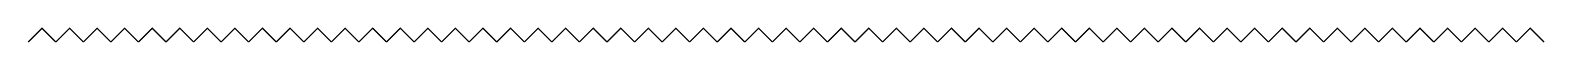
\begin{tikzpicture}[scale=0.35]
\foreach \x in {1,...,55}{
	\draw (\x,-0.25)--(\x+0.5,0.25)--(\x+1,-0.25);
}
\end{tikzpicture}
}

\usepackage{tikz}

\title{\textbf{ Examples: Theta Functions and Poisson Summation}}
\author{John D Mangual}
\date{}
\begin{document}

\fontfamily{qag}\selectfont \fontsize{25}{30}\selectfont

\maketitle

\fontfamily{qag}\selectfont \fontsize{12}{10}\selectfont

\noindent On the one hand, there are many people who know all sorts of things about theta functions.  David Mumford wrote 3 volumes.  They are going to my working examples of modular forms.\footnote{There is also an excellent discussion of Theta Functions and String Theory and Riemann surfaces by the Verlinde brothers, some of which is formalized by Beauville.  There's even a page or two in Feynman's \textbf{Statistical Mechanics}. } \\ \\
\textbf{Ex \#1} Show that if $u(x)$ is a spherical harmonic of degree $\ell$ the generalized theta function
$$ \theta(z; u) = \sum_{m \in \mathbb{Z}^3} u(m) e^{z|m|^2} $$
is a holomorphic cusp form for $\Gamma_0(4)$ of weight $3/2 + \ell$ as long as $\ell \geq 1$.  This will already keep me busy for some time.  The coefficients of this Fourier series are averages over the sphere:
$$  \frac{1}{r_3(n)} \sum_{\xi_1^2 + \xi_2^2 + \xi_3^2 = n} u(\xi) \ll   n^{- 1/28}$$
\textbf{Ex \#2} Show Duke's bound for any exponent $n^\alpha$ with $\alpha < 0$.  Could be $\frac{1}{28}$ or $\frac{1}{100}$\dots Anything.  \\ \\ \\
If I knew what a $\Gamma_0(4)$ holomorphic cusp form was, I might be able to credit Goro Shimura's 1973 paper.  However, he has also written some recent graduate level texts with chaptrs on half-integer weight modular forms.  \\ \\ 
The fraction $\frac{1}{28}$ falls out of difficult calculations involving Kloosterman sums, which I am not going to cite or reproduce.  Therefore, I might expect these bounds to be slightly worse -- if I achieve anything at all.   Instead, I will emphasize elementary\footnote{Duke and Iwaniec also felt there arguments were elementary.  I am sure Duke and Shimura are correct.} computations.\\ \\ 
There are a few easy cases $u(\xi) = 1$ is the spherical harmonic of degree 0 -- it is excluded from discussion.  In fact, $\ell \geq 1$ and $n \gg 1$ should be very large.  Yet:
$$  \frac{1}{r_3(n)} \sum_{\xi_1^2 + \xi_2^2 + \xi_3^2 = n} 1 = 1  $$
and $\xi(x,y,z) = x$ is an odd function.  So that $x^2 + y^2 + z^2 = n$ should have a solution $(x,y,z)$ and $(-x,y,z)$.  Therefore, any odd function such as $u(x,y,z) = x$ should have a vanishing average.  \\ \\
The first non-trivial case -- and we're a far cry from proving Ex \#1 or Ex \#2 -- is $u(x) = x_1^2$ ( notice $u(x) = x_1 x_2$ also vanishes ).  This is not to be understimated that we can switch signs.
$$ (\pm x_1)^2 + (\pm x_2)^2 + (\pm x_3)^2 = n $$
However let's not to forget to try far more basic approaches such as the Hasse Princple.\footnote{Or the mean value theorem! Let $f: \mathbb{R}^3 \to \mathbb{R}$ show that $|\frac{1}{6}\sum_{k \in \{1,2,3\}} f(x \pm dx_k) - f(x)|\ll \partial f (x)$ (this is ambiguous)}

\newpage
%\fontfamily{qag}\selectfont \fontsize{12}{10}\selectfont


\begin{thebibliography}{}

\item Emil Artin and George Whaples \textbf{Axiomatic characterization of fields by the product formula for valuations} Bull. Amer. Math. Soc.
Volume 51, Number 7 (1945), 469-492.




\end{thebibliography}



\end{document}